\chapter{Практические задания}

\begin{enumerate}[wide=0pt]
\item \textit{Составить диаграмму вычисления следующих выражений::}
\begin{enumerate}[label=\arabic*)]
	\item \lstinline {(equal 3 (abs - 3))}
	\item \lstinline {(equal (+ 1 2) 3)}
	\item \lstinline {(equal (* 4 7) 21)}
	\item \lstinline {(equal (* 2 3) (+ 7 2))}
	\item \lstinline {(equal (- 7 3) (* 3 2))}
	\item \lstinline {(equal (abs (- 2 4)) 3))}
	
\end{enumerate}


\begin{figure}[ht!]
	\centering
	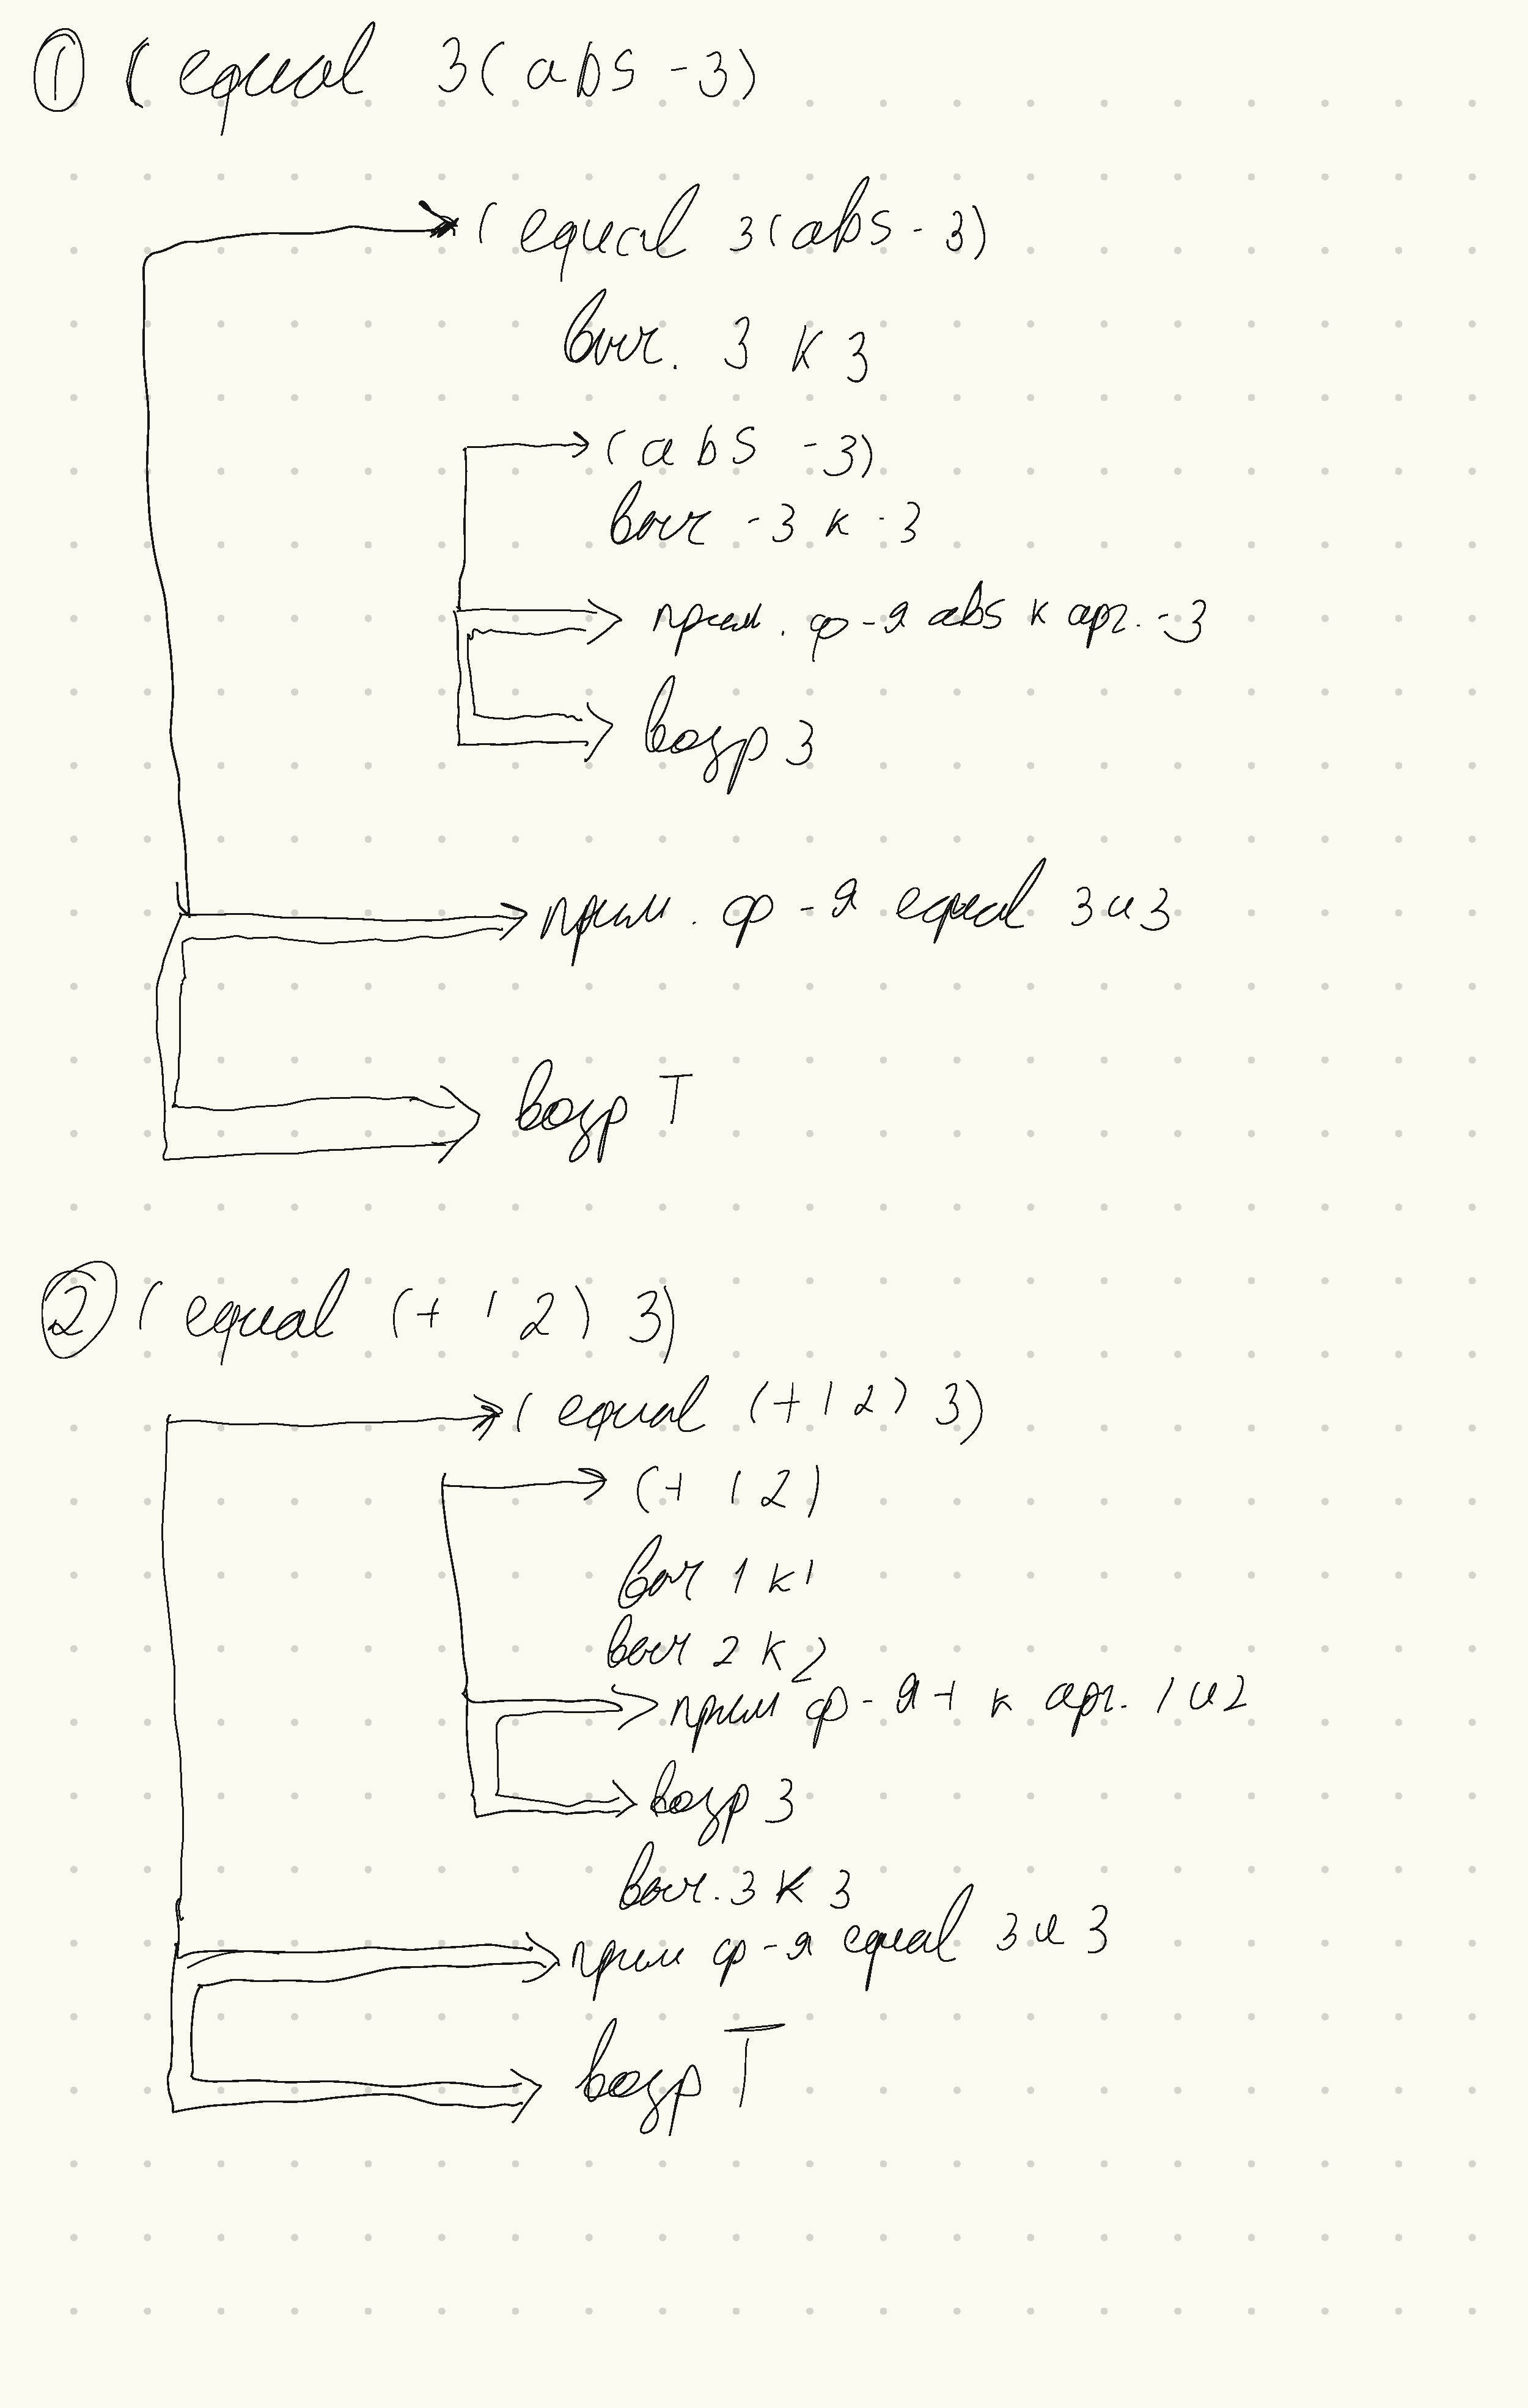
\includegraphics[width=1\linewidth]{assets/task1/1.pdf}
	\caption{Списочные ячейки. Задание 1}
\end{figure}
\FloatBarrier



\item  \textit{Написать функцию, вычисляющую гипотенузу прямоугольного}

\end{enumerate}